\documentclass{article}
\usepackage{graphicx}
\begin{document}

\section{Introduction}
This report covers Bayesian Neural Network experiments:
\begin{itemize}
\item Sinusoidal regression task
\item PovertyMap satellite imagery analysis
\item Comparison of Laplace approximation and Bayesian-Torch (SVI with Flipout)
\end{itemize}

\section{Methods}
\subsection{Laplace Approximation}
\begin{itemize}
\item Post-hoc Gaussian approximation around MAP estimate
\item Uses full covariance for last layer
\item GLM predictive with 2000 samples
\item Hyperparameters tuned by minimizing NLL on validation set
\end{itemize}

\subsection{Bayesian-Torch with Flipout SVI}
\begin{itemize}
\item Learns variational posterior via SVI
\item Uses Flipout estimator to lower variance
\item MC sampling for predictive distribution (50-100 samples)
\item Initialized from MAP via MOPED
\end{itemize}

\section{Results}
\subsection{Sinusoidal Regression}
\begin{itemize}
\item Network: Linear(1,50) -> Tanh -> Linear(50,1)
\item Compared MAP baseline, Laplace-Torch, Bayesian-Torch
\item Tracked RMSE, NLL, Calibration Error, training/inference times
\end{itemize}

\subsection{PovertyMap (WILDS)}
\begin{itemize}
\item ResNet-18 adapted for 8-channel satellite images
\item 5-fold cross-validation across country splits (Folds A-E)
\item Evaluated RMSE, NLL, Regression Calibration Error
\item Compared Laplace (full last-layer + GLM) vs Bayesian-Torch (Flipout + SVI)
\end{itemize}

\section{Libraries Overview}
From CSV file:
\begin{itemize}
\item BI: based on NumPyro/TFP (JAX)
\item PyMC: PyTensor, Variational Inference / MCMC
\item Bayes-Torch: PyTorch, stochastic VI (BBB)
\item Laplace-Torch: PyTorch, Laplace approximation
\item TyXe: PyTorch, VI / MCMC
\item BLiTZ: PyTorch, VI BBB
\end{itemize}

\section{Figures}
\begin{figure}[h]
\centering
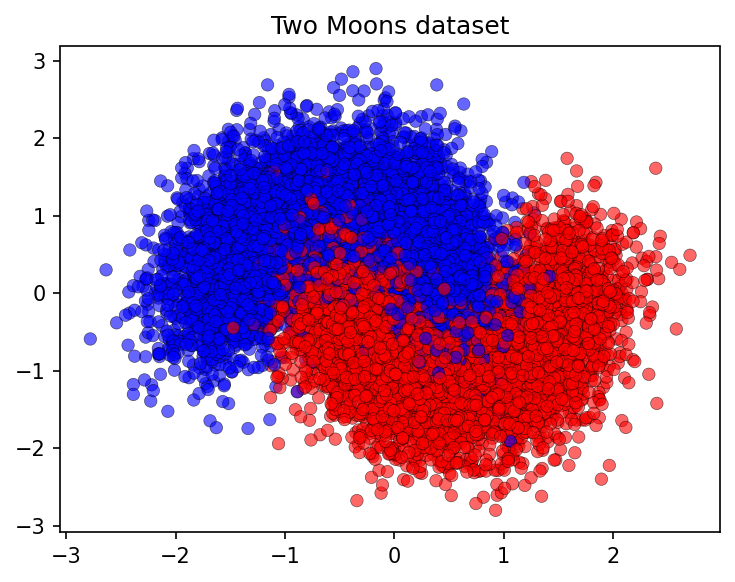
\includegraphics[width=0.45\textwidth]{./laplace_torch/figures/01_raw_dataset.png}
\caption{Raw sinusoidal dataset}
\end{figure}

\begin{figure}[h]
\centering
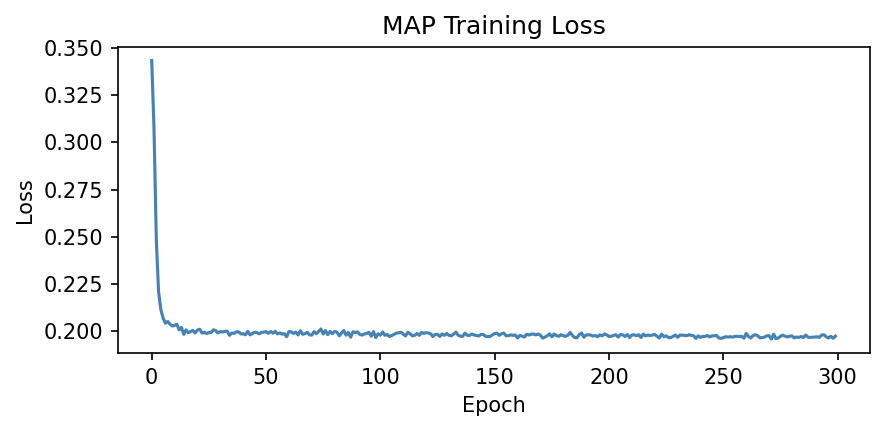
\includegraphics[width=0.45\textwidth]{./laplace_torch/figures/02_map_training_loss.png}
\caption{MAP training loss}
\end{figure}

\end{document}